\documentclass[12pt]{article}
\setlength\parindent{0pt}
\usepackage{fullpage}
\usepackage{amsmath}
\usepackage{graphicx}
\usepackage[left=2cm, right=2cm, top=1.5cm, bottom=1cm]{geometry}
%\usepackage[margin=0.5in, paperwidth=13.5in, paperheight=8.4375in]{geometry}
\setlength{\parskip}{4mm}
\def\LL{\left\langle}   % left angle bracket
\def\RR{\right\rangle}  % right angle bracket
\def\LP{\left(}         % left parenthesis
\def\RP{\right)}        % right parenthesis
\def\LB{\left\{}        % left curly bracket
\def\RB{\right\}}       % right curly bracket
\def\PAR#1#2{ {{\partial #1}\over{\partial #2}} }
\def\PARTWO#1#2{ {{\partial^2 #1}\over{\partial #2}^2} }
\def\PARTWOMIX#1#2#3{ {{\partial^2 #1}\over{\partial #2 \partial #3}} }
\newcommand{\BE}{\begin{displaymath}}
\newcommand{\EE}{\end{displaymath}}
\newcommand{\BNE}{\begin{equation}}
\newcommand{\ENE}{\end{equation}}
\newcommand{\BEA}{\begin{eqnarray}}
\newcommand{\EEA}{\nonumber\end{eqnarray}}
\newcommand{\EL}{\nonumber\\}
\newcommand{\la}[1]{\label{#1}}
\newcommand{\ie}{{\em i.e.\ }}
\newcommand{\eg}{{\em e.\,g.\ }}
\newcommand{\cf}{cf.\ }
\newcommand{\etc}{etc.\ }
\newcommand{\Tr}{{\rm tr}}
\newcommand{\etal}{{\it et al.}}
\newcommand{\OL}[1]{\overline{#1}\ } % overline
\newcommand{\OLL}[1]{\overline{\overline{#1}}\ } % double overline
\newcommand{\OON}{\frac{1}{N}} % "one over N"
\newcommand{\OOX}[1]{\frac{1}{#1}} % "one over X"



\begin{document}
\pagenumbering{gobble}
\Large
\centerline{\sc{Recitation Questions}}
\normalsize
\centerline{\sc{5 March}}

Today's recitation has two problems. The first is designed to teach you how to handle objects that move on a slope. First, you will do
it in the easier way, using a rotated coordinate system where $x$ is the direction parallel to the hill and $y$ is the direction perpendicular to it. If you have time, you will also approach it using the conventional coordinate system, where $x$ and $y$ are horizontal and vertical, and compare the approaches. 

The second problem involves two objects that are roped together. It will teach you how to handle situations like this where two objects have accelerations that are related, but not necessarily equal.

Your recitation evaluation today will be a brief Blackboard quiz; it should take you about three minutes to complete.

\begin{center}
	\underline{\hspace{0.7\textwidth}}
\end{center}

These problems, like all others for the next few weeks involving Newton's second law, can be approached as follows:

\begin{enumerate}
	\item Draw a cartoon of the situation, and draw force diagrams for all objects.
	\begin{itemize}
		\item Choose a coordinate system (which way is $x$ and which way is $y$?)
		\item If you have any forces that aren't aligned with $x$ and $y$, do trigonometry to find their $x-$ and $y-$components
		\item Remember, only physical pushes and pulls are forces -- not abstract ideas like ``acceleration'' or ``net force''
	\end{itemize}
	\item Write down Newton's law of motion $\sum \vec F = m \vec a$ for each object, along each axis that is relevant
	\begin{itemize}
		\item If your force diagrams are clear, you can read these equations straight off your diagrams
	\end{itemize}
	\item Substitute in things you know; solve for things you don't
	\begin{itemize}
		\item If you have more than one object, some forces may be equal by Newton's third law; you can substitute this in
		\item You may know things about the acceleration of the object in different directions, or the forces on it
		\item Solve the resulting system of equations by substitution
	\end{itemize}


\end{enumerate}

\newpage




Tux the penguin slides down a frictionless icy hill; the hill is inclined at an angle $\theta$. In this problem, you will 
calculate the penguin's acceleration. First, let's do it with the rotated coordinate system -- the easier approach.

Here you will need to draw {\it large} diagrams, since you will need to label and think carefully about your coordinate systems and vector components, drawing triangles on top of them and doing trigonometry. If you spend as much as 10-15 minutes on this step, that is okay; it is very important to get right. Please call over your TA/coach and discuss this with them.



\bigskip


a) Draw a cartoon of the problem, and label your coordinate system.


\vspace{2in}

	b) Draw a force diagram for the penguin. (Draw this one large, since you will need to construct a right triangle with one of the forces as its hypotenuse to break it into components.) Before you go onto the next page, once you and your group agree on the force diagram, copy it onto your own paper. You'll need it again.



\vspace{2in}


\newpage

c) Write down Newton's second law in both directions -- that is, $\sum F_x = ma_x$ and $\sum F_y = ma_y$. If you have any forces that don't lie along the $x$ or $y$ directions, use trigonometry to break them into components.

\vspace{1.7in}

d) This will result in two equations with three unknowns: $a_x$, $a_y$, and $F_N$. However, in this problem, $a_x$ and $a_y$ are related. What is their relation? This should reduce you to two equations and two unknowns; write them below.
\vspace{1.7in}

e) Solve those equations to find the acceleration of the penguin. Use trigonometry to find the magnitude of $\vec a$.

\newpage

If you have at least 35 minutes left in the recitation section, try solving the problem using the conventional coordinate system, where $x$ is horizontal and $y$ is vertical. Otherwise, skip ahead to the problem with the pulleys. Here, again:

a) Draw a cartoon of the problem, and label your coordinate system. 

\vspace{2.5in}

b) Draw a force diagram for the penguin.  If you have any forces that don't lie along the $x$ or $y$ directions, use trigonometry to break them into components. 


\newpage

c) Write down Newton's second law in both directions -- that is, $\sum F_x = ma_x$ and $\sum F_y = ma_y$. 

This will require some thought: you will need to figure out the components of the 
penguin's weight in the $x$ and $y$ directions. Call over your TA or coach to check your work when you are done.

\vspace{3in}


d) This will result in two equations with three unknowns: $a_x$, $a_y$, and $F_N$. However, a little thought will
tell you what one of these is. What is it? This should reduce you to two equations and two unknowns; write them below. Once you and your group agree on them, copy them onto your own paper.

\vspace{2in}
\newpage
e) Solve those equations to find the acceleration of the penguin.

\vspace{2in}

f) Discuss the difference in the two approaches. In one, you aligned your coordinate system with gravity, and in the other, you aligned your coordinate system with the direction that you knew the penguin would accelerate in. Which was easier? Which 
should you adopt for future problems? Invite your TA or coach over to join your conversation.

\newpage
\begin{minipage}{0.7\textwidth}
Two weights of mass $m_1$ and $m_2$ are attached to either end of a string. This string is passed over a light frictionless pulley, as shown in the image.
Clearly the heavier mass will go down and the lighter one will go up, but at what rate? In this problem, you will calculate their acceleration.

\bigskip\bigskip

a) What do you expect the system to do if one of the masses is much heavier than the other? What do you expect if the
two masses are equal?


\end{minipage} \hfill
\begin{minipage}{0.3\textwidth}
\begin{center}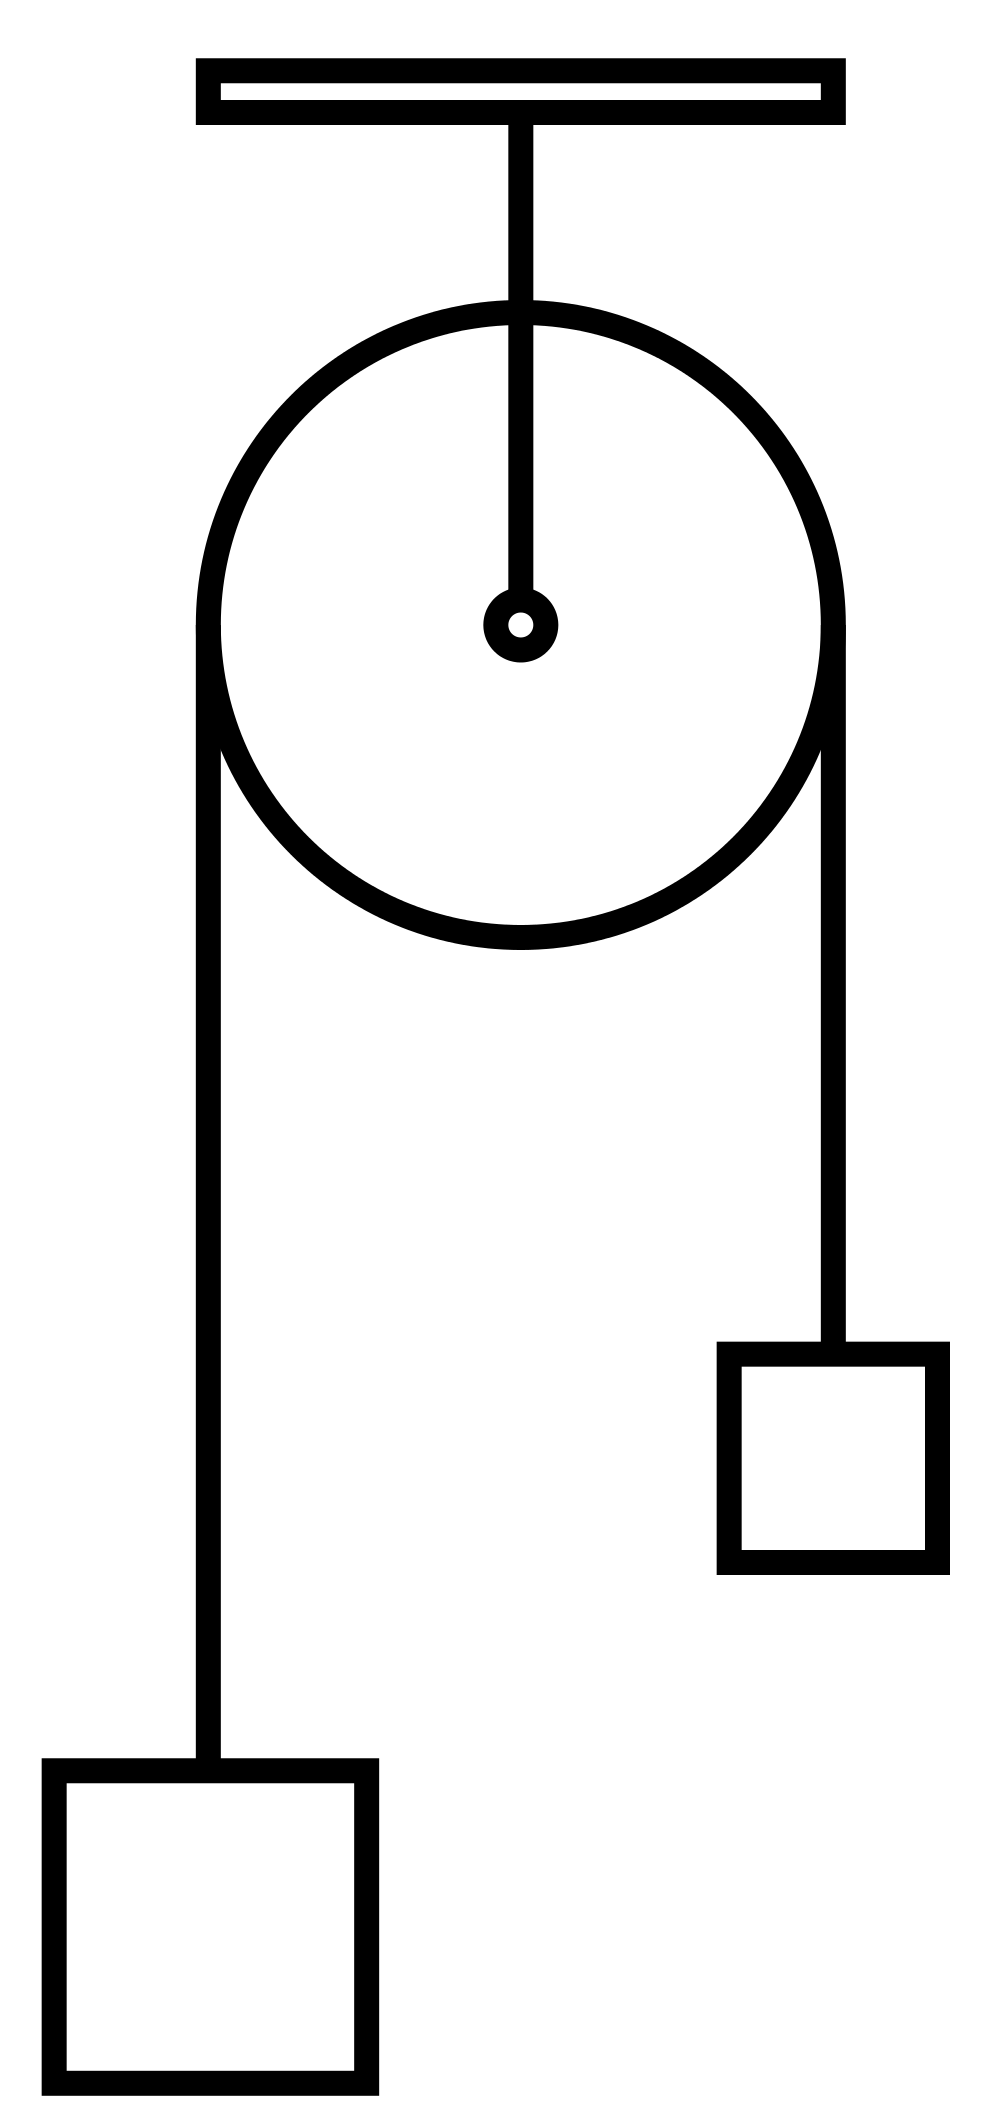
\includegraphics[width=0.3\textwidth]{atwood.png}
\end{center}
\end{minipage} \hfill




b) Draw force diagrams for both objects. Label your choice of coordinate system separately for each object -- you don't have to choose the same coordinate system for each! 

\vspace{2in}

c) State Newton's law for both objects. Note that their accelerations aren't necessarily the same, depending on your choice of coordinate system, so you should introduce separate variables $a_1$ and $a_2$ for both. The tension forces
{\it are} the same.

\newpage

d) Since you have two objects, you have two copies of Newton's law. However, you have three unknowns: $T$, $a_1$, and $a_2$. What other statement can you make about the accelerations that lets you solve the system?

\vspace{3in}

e) Actually solve the system, giving values of $a_1$ and $a_2$ in terms of $m_1$, $m_2$, and $g$. Then, translate 
your expressions for $a_1$ and $a_2$ into words. (Your TA and coaches can help with this.) Does your result make sense?
Does it agree with your predictions in part (a)? 

\end{document}
